\section{Multigrid Methods}
Multigrid methods have been designed to accelerate the convergence of iterative methods by eliminating certain error components on a so-called coarser representation of the original problem.
While the basic iterative methods discussed in the last section are applicable to many PDE-based problems, in practice, their speed of convergence is often insufficient, which means that a large number of iterations is required until an acceptable approximation accuracy can be attained. 
The main reason for this behavior is that these methods are only efficient in the reduction of certain error components, while others remain mostly unaffected~\cite{briggs2000multigrid}.
This can be best understood by considering the effect of a stationary iterative method on oscillatory errors of different frequency.
For this purpose, we consider the one-dimensional Laplace equation
\begin{equation}
		\begin{split}
			- \dv[2]{x} u(x) & = 0 \quad \forall x \in (0, 1) \\
			u(0) = u(1) & = 0,
		\end{split}
		\label{eq:1D-laplace-model}
\end{equation}
which is discretized using the three-point stencil
\begin{equation}
	\Delta_h^{(3, 1)} = \frac{1}{h^2}\begin{bmatrix}
		-1 & 2 & -1
	\end{bmatrix}.
\end{equation} 
Figure~\ref{fig:different-error-components-jacobi} shows different periodic error components before and after the application of 100 Jacobi steps with a relaxation factor $\omega = 2/3$.
Note that the frequency of change differs between each of the three cases, whereas the amplitude of the error is always the same.

\begin{figure}
	\centering
	\begin{subfigure}[b]{0.45\textwidth}
		\centering
		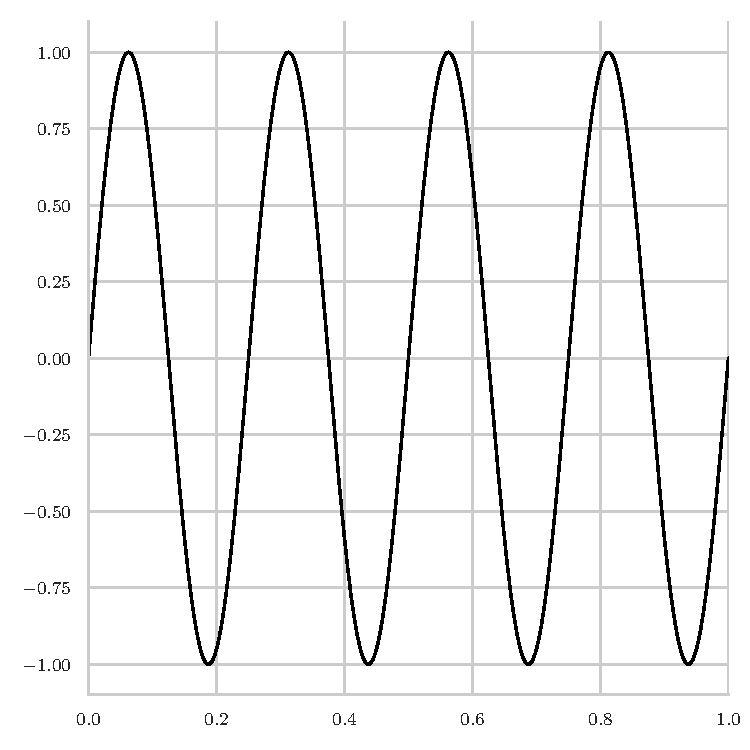
\includegraphics[width=\textwidth]{figures/jacobi_initial_error2.pdf}
		%\caption{Initial Error}
	\end{subfigure}
	\hfill
	\begin{subfigure}[b]{0.45\textwidth}
		\centering
		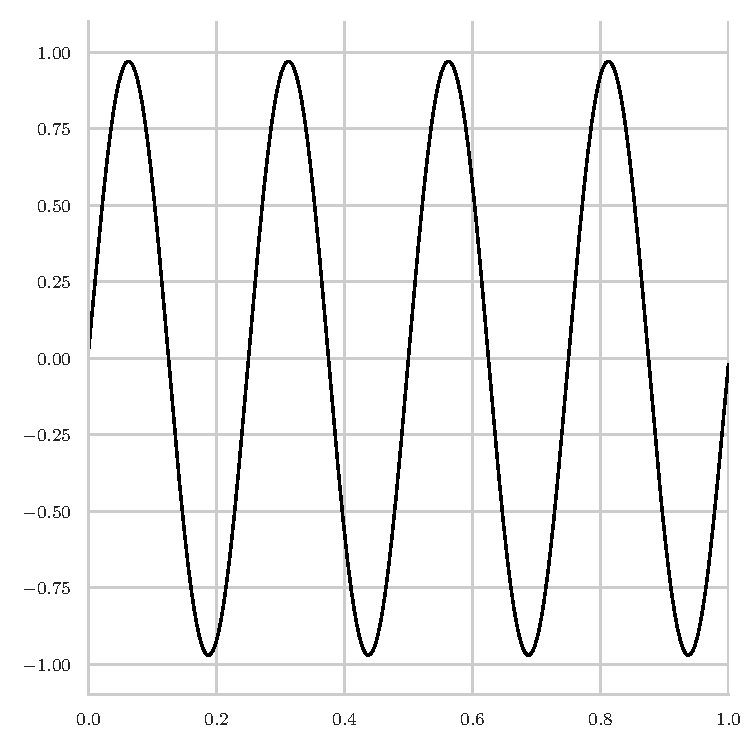
\includegraphics[width=\textwidth]{figures/jacobi_final_error2.pdf}
		%\caption{Error after 100 Steps of weighted Jacobi}
	\end{subfigure}
	\begin{subfigure}[b]{0.45\textwidth}
	\centering
	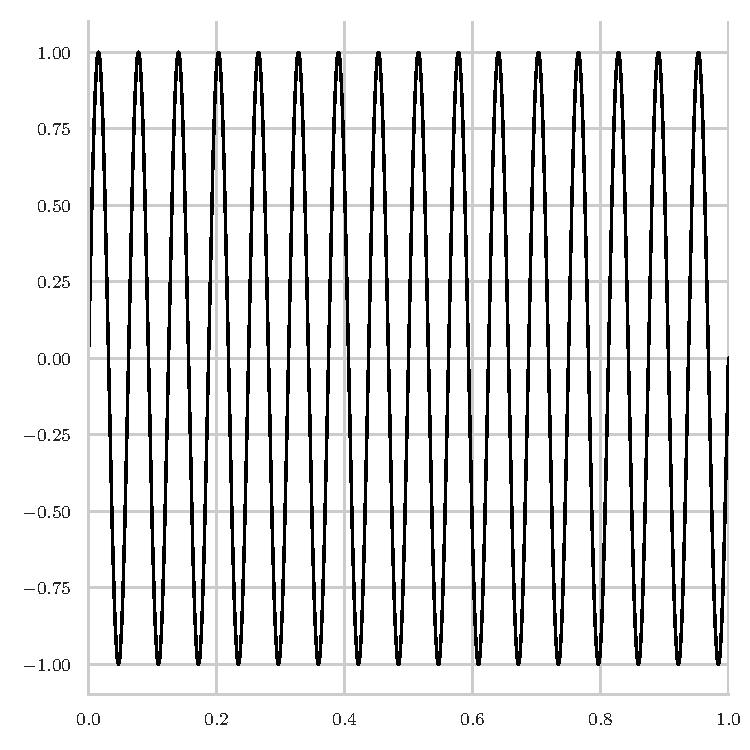
\includegraphics[width=\textwidth]{figures/jacobi_initial_error4.pdf}
	%\caption{Initial Error}
	\end{subfigure}
	\hfill
	\begin{subfigure}[b]{0.45\textwidth}
		\centering
		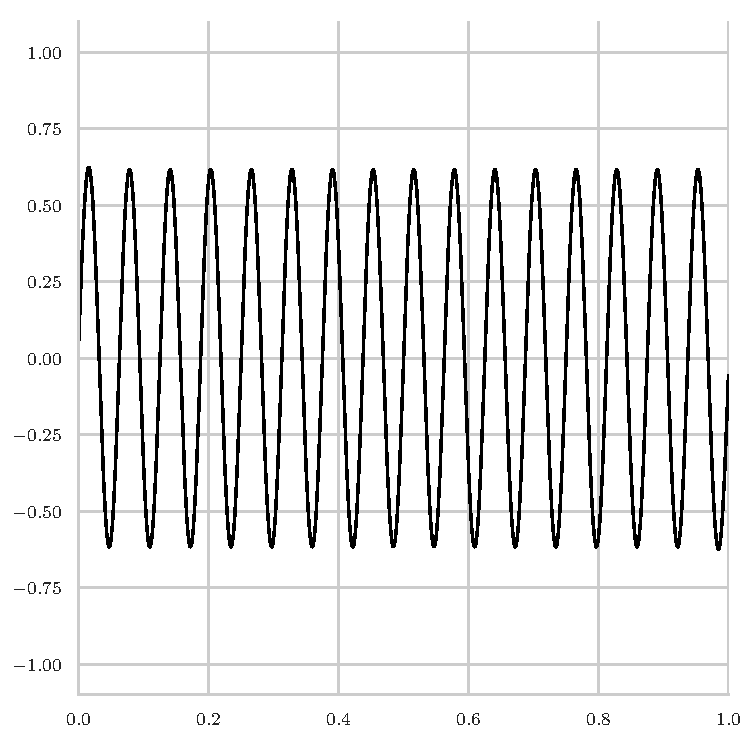
\includegraphics[width=\textwidth]{figures/jacobi_final_error4.pdf}
		%\caption{Error after 100 Steps of weighted Jacobi}
	\end{subfigure}
	\begin{subfigure}[b]{0.45\textwidth}
		\centering
		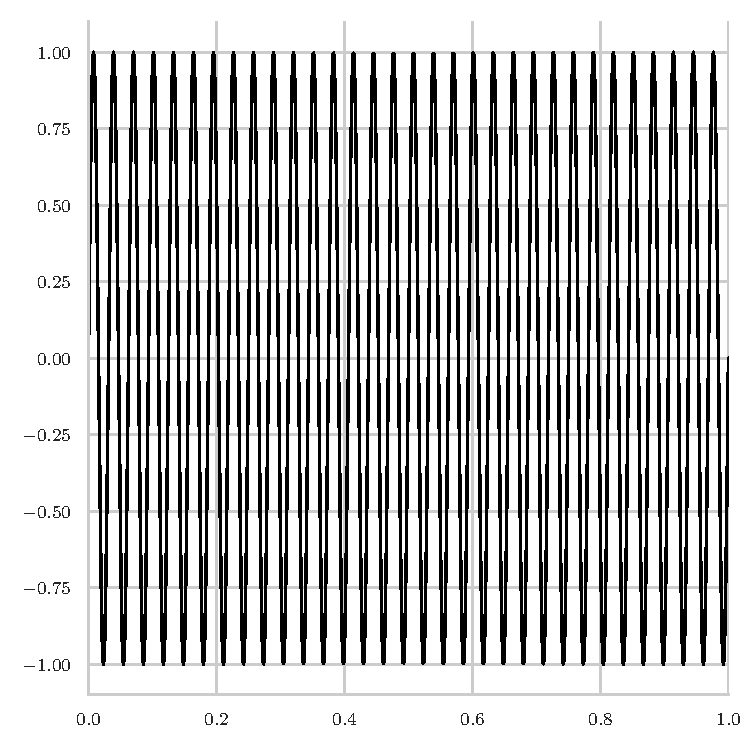
\includegraphics[width=\textwidth]{figures/jacobi_initial_error5.pdf}
		%\caption{Initial Error}
	\end{subfigure}
	\hfill
	\begin{subfigure}[b]{0.45\textwidth}
		\centering
		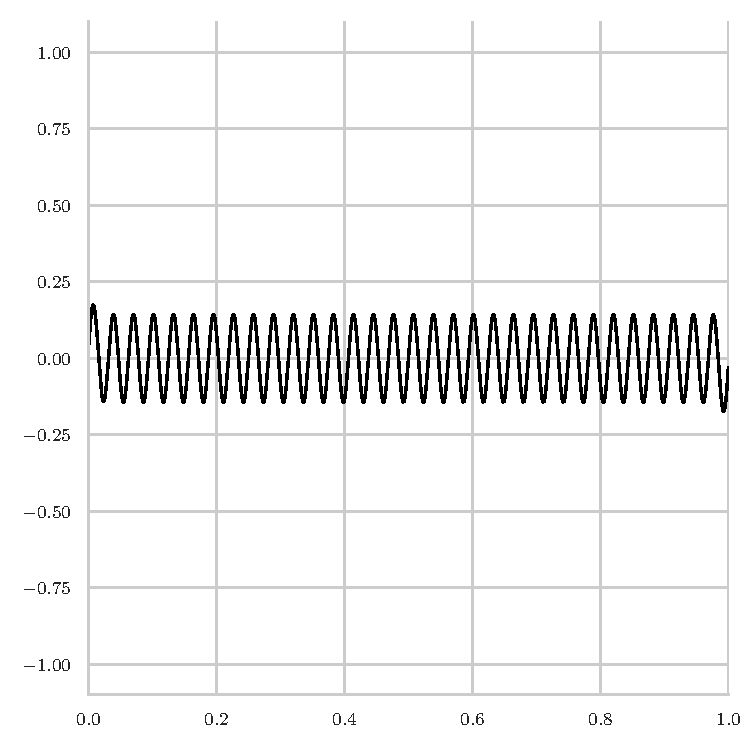
\includegraphics[width=\textwidth]{figures/jacobi_final_error5.pdf}
		%\caption{Error after 100 Steps of weighted Jacobi}
	\end{subfigure}
	\caption{Different error components before and after 100 steps of weighted Jacobi with $\omega = 2/3$.}
	\label{fig:different-error-components-jacobi}
\end{figure}
\begin{figure}
	\begin{subfigure}[b]{0.45\textwidth}
	\centering
	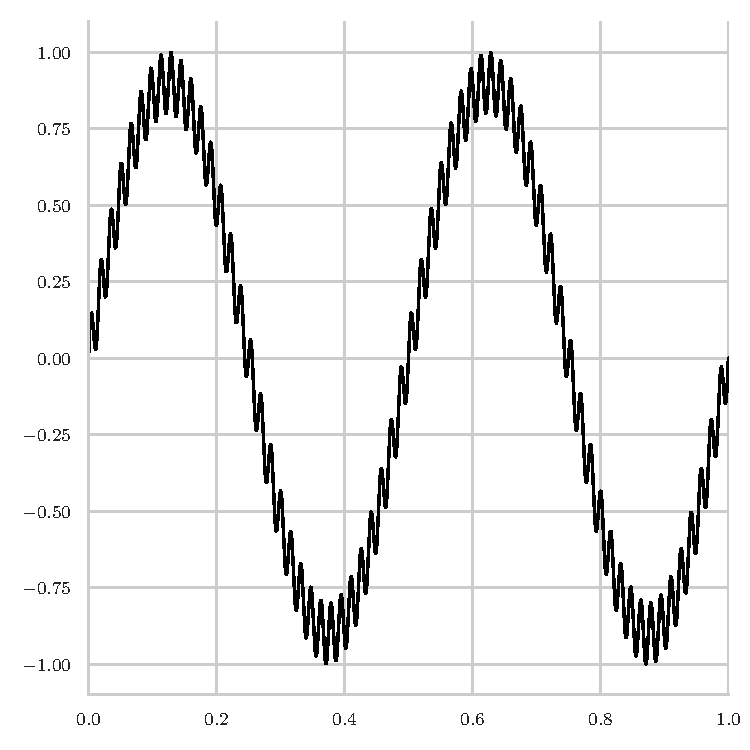
\includegraphics[width=\textwidth]{figures/jacobi_initial_error6.pdf}
\end{subfigure}
\hfill
\begin{subfigure}[b]{0.45\textwidth}
	\centering
	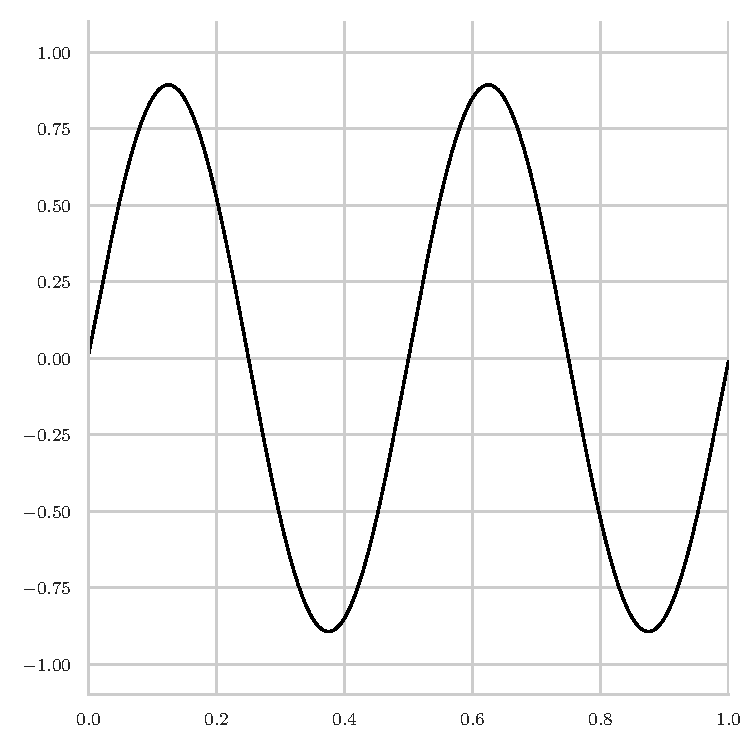
\includegraphics[width=\textwidth]{figures/jacobi_final_error6.pdf}
\end{subfigure}
	\caption{Combination of two error components before and after 100 steps of weighted Jacobi with $\omega = 2/3$.}
\label{fig:combined-error-jacobi}
\end{figure}

